%%%%%%%%%%%%%%%%%%%%%%%%%%%%%%%%%%%%%%%%%%%%%%%%%%%%%%%%%%%%%%%%%%%%%%%%%%%

\documentclass[a4paper,oneside,12pt]{article}
\usepackage{mystyle}

\begin{document}

\title{\Large\bf Factoring a quadratic function}
\author{%%
  Minh Van Nguyen \\
  \url{mvngu@gmx.com}
}
\date{\today}
\maketitle

\noindent
This document will show you how to factorise a quadratic function.
One reason why you would factorise a quadratic function is so that you
can determine the roots of the function without using the quadratic
formula.  To factorise an expression means to write the expression as
the product of two or more expressions.  In the case of the number
$6$, you can factorise $6$ by writing it as the product of $2$ and
$3$.  Hence the integer $6$ can be written in factored form as
\[
6
=
2 \times 3
\]
and you say that $2$ and $3$ are factors of $6$.  As another example,
you can write $60$ in factored form as $60 = 3 \times 20$.  You can
also factorise $20$ to get $20 = 4 \times 5$ and therefore $60$ can be
factorised as
\[
60
=
3 \times 4 \times 5.
\]
As can be seen from the above examples, factorising an integer
involves writing the integer as the product of two or more integers.
The factors are usually prime integers.  A factorisation such as
$5 = 1 \times 5$ is correct because $5$ is a prime and has no positive
factors other than $1$ and $5$.  The factored form
$5 = 1 \times 5 \times 1$ is also correct, but that's cheating.


%%%%%%%%%%%%%%%%%%%%%%%%%%%%%%%%%%%%%%%%%%%%%%%%%%%%%%%%%%%%%%%%%%%%%%%%%%%

\section{Factoring when $c = 0$}

What about factoring quadratic functions?  Let's start with quadratic
functions of the form $f(x) = ax^2 + bx$, where $a$ and $b$ are any
real numbers such that $a \neq 0$.  Note that $c = 0$ and so the
vertical intercept of $f(x)$ is the point $\tuple{0}{0}$.  Use the
distributive laws to write $f(x)$ in the factored form
%%
\begin{equation}
\label{eqn:factorise_axx_bx}
f(x)
=
(ax + b)x
\end{equation}
%%
and you can see that $f(x)$ has the factors $x$ and $ax + b$.  Looking
at the factored form~\eqref{eqn:factorise_axx_bx}, the roots of $f(x)$
are $x = 0$ and $x = -b/a$.  But how did you get those numbers?  To
calculate the roots of $f(x)$ means to determine all values of $x$
such that the expression $f(x) = 0$ is true.  In other words, you want
to determine all values of $x$ such that the expression
%%
\begin{equation}
\label{eqn:roots_of_axx_bx}
(ax + b)x
=
0
\end{equation}
%%
is true.  Expression~\eqref{eqn:roots_of_axx_bx} tells you that there
are two numbers, i.e.~$x$ and $ax + b$, whose product is zero.  You
have two cases:
%%
\begin{packedenumeral}
\item If $x = 0$, then \Expression{eqn:roots_of_axx_bx} is true
  because zero multiplied by another number is zero.  So one root of
  $f(x)$ is $x = 0$.

\item If $ax + b = 0$, then \Expression{eqn:roots_of_axx_bx} is also
  true.  But for which values of $x$ would you have $ax + b = 0$?
  Solving the latter expression for $x$ shows that $x = -b / a$.
  Substitute the last expresssion into~\eqref{eqn:roots_of_axx_bx}
  produces
  %%
  \begin{align*}
  \squarebracket*{
    a \parenthesis*{-\frac{b}{a}}
    +
    b
  }
  \parenthesis*{-\frac{b}{a}}
  &=
  (-b + b)
  \parenthesis*{-\frac{b}{a}} \\[4pt]
  &=
  0 \times \parenthesis*{-\frac{b}{a}} \\[4pt]
  &=
  0
  \end{align*}
  %%
  which is true.  Hence you have found that $x = -b / a$ is another
  root of $f(x)$.
\end{packedenumeral}
%%
By writing $f(x)$ as the factored form~\eqref{eqn:factorise_axx_bx}
you can easily determine the roots of $f(x)$ without using the
quadratic formula.  The above discussion is summarised in the
following theorem.

\begin{theorem}
\label{thm:quadratic_function_vertical_intercept_zero}
Consider the quadratic function $f(x) = ax^2 + bx$, where $a$ and $b$
are any real numbers such that $a \neq 0$.  The roots of $f(x)$ are
\[
x = 0
%%
\qquad
\text{and}
\qquad
%%
x = -\frac{b}{a}.
\]
\end{theorem}

\begin{example}
\label{eg:AmazingCar}
\textbf{AmazingCar.}
At a particular toy store, the sales of a toy called AmazingCar is
given by the sales function $S(x) = -3x + 40$.  Here $x$ represents
the price in dollars of each unit of AmazingCar and so $x$ is the unit
price.  The sales function $S(x)$ represents the number of units of
AmazingCar sold during a week.
%%
\begin{packedenum}
\item\label{subeg:AmazingCar_graph_sales_function}
  Produce a graph of the sales function.  Use the graph to help you
  explain the sales function.  Identify the unit prices at which the
  number of units of AmazingCar sold is highest and lowest.

\item\label{subeg:AmazingCar_revenue_function}
  Derive an expression for the revenue from selling units of
  AmazingCar during a particular week.  Produce a graph of the revenue
  function.

\item\label{subeg:AmazingCar_price_zero_revenue}
  At which unit prices would the revenue from selling units of
  AmazingCar be zero dollars during a week?
\end{packedenum}
\end{example}

\begin{solution}
\solutionpart{subeg:AmazingCar_graph_sales_function}
\Figure{fig:AmazingCar_sales} shows a graph of the sales function
$S(x)$.  The graph shows that as the price for each unit of AmazingCar
increases the lower is the number of units sold during a week.  In
other words, the lower is the unit price the higher is the number of
units sold during the week.  This sounds reasonable because as the
price of something decreases you would expect to sell more of the
product.  Note the two points on the graph that show the lowest and
highest number of units sold.  These are the intercepts of the axes.
The horizontal intercept is the point $\tuple{\frac{40}{3}}{0}$, which
tells you that when the unit price is approximately $\$13.33$ zero
units of AmazingCar would be sold per week.  The lowest number of
units sold per week is zero.  The vertical intercept $\tuple{0}{40}$
tells you that when the unit price is zero dollars~(each unit of
AmazingCar is given away free of charge), the number of units sold per
week is $40$, which is also the highest number of units sold per
week.

\begin{figure}[!htbp]
\centering
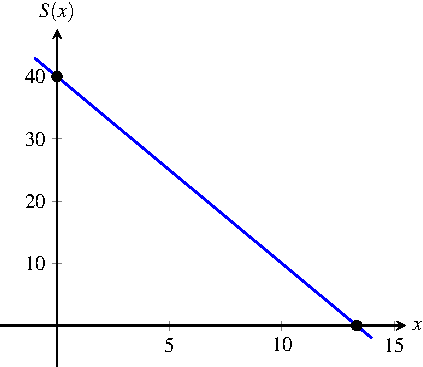
\includegraphics[scale=1.1]{image/10/amazingcar-sales.pdf}
\caption{%%
  Graph of the sales function $S(x) = -3x + 40$ for AmazingCar.  Here
  $x$ represents the unit price in Australian dollars and $S(x)$
  represents the number of units of AmazingCar sold at $x$ dollars
  per unit.
}
\label{fig:AmazingCar_sales}
\end{figure}

\solutionpart{subeg:AmazingCar_revenue_function}
Since $x$ is the unit price and $S(x)$ represents how many units were
sold during a week, the revenue from selling AmazingCar is the
expression
\[
R(x)
=
x S(x)
=
x(-3x + 40).
\]
The revenue function is graphed in \Figure{fig:AmazingCar_revenue}.

\begin{figure}[!htbp]
\centering
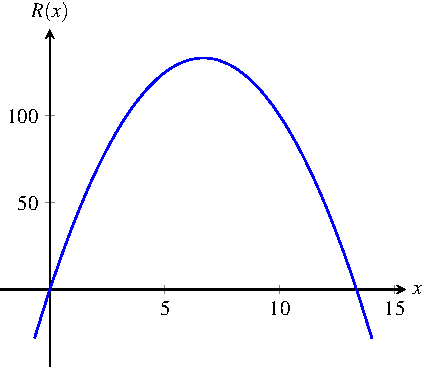
\includegraphics[scale=1.1]{image/10/amazingcar-revenue.pdf}
\caption{%%
  Graph of the revenue function $R(x) = x(-3x + 40)$ for AmazingCar.
  The function $R(x)$ represents the revenue~(in dollars) from selling
  units of AmazingCar during a week at $x$ dollars per unit.
}
\label{fig:AmazingCar_revenue}
\end{figure}

\solutionpart{subeg:AmazingCar_price_zero_revenue}
\Figure{fig:AmazingCar_revenue} shows that you have two unit prices at
which the revenue from selling AmazingCar would be zero dollars during
a week.  Those particular two unit prices are the roots of $R(x)$.
You can use the quadratic formula to determine the roots of $R(x)$.
However, note that you can use the distributive laws to write the
revenue function as
%%
\begin{equation}
\label{eqn:AmazingCar_revenue_function_distributive}
R(x)
=
-3x^2 + 40x.
\end{equation}
%%
You then use \Theorem{thm:quadratic_function_vertical_intercept_zero}
to conclude that the roots of $R(x)$ are $x = 0$ and
\[
x
=
-\frac{40}{-3}
=
\frac{40}{3}.
\]
In other words, the revenue during a week from selling units of
AmazingCar would be zero dollars if the unit prices were either zero
dollars or approximately $\$13.33$.
\end{solution}

\begin{exercise}
\textbf{More AmazingCar.}
You will further explore \Example{eg:AmazingCar}.
%%
\begin{packedenum}
\item\label{subeg:AmazingCar_roots_quadratic_formula}
  Use the quadratic formula to verify the roots of the revenue
  function.

\item\label{subeg:AmazingCar_maximum_revenue}
  Determine the unit price that would result in maximum revenue for a
  week from selling units of AmazingCar.
\end{packedenum}
\end{exercise}

\ifbool{showSolution}{
\begin{solution}
\solutionpart{subeg:AmazingCar_roots_quadratic_formula}
Apply the quadratic formula on the revenue
function~\eqref{eqn:AmazingCar_revenue_function_distributive} to see
that the roots of $R(x)$ are given by the expression
%%
\begin{align*}
x
&=
\frac{
  -40 \pm \sqrt{40^2 - 4(-3)(0)}
}{
  2(-3)
} \\[4pt]
&=
\frac{
  -40 \pm 40
}{
  -6
}.
\end{align*}
Thus the roots of $R(x)$ are
\[
x
=
\frac{-40 + 40}{-6}
=
0
\]
and
\[
x
=
\frac{-40 - 40}{-6}
=
\frac{40}{3}
\]
which are the same as what you got in \Example{eg:AmazingCar}.

\solutionpart{subeg:AmazingCar_maximum_revenue}
The maximum revenue is located at the vertex in the graph of $R(x)$.
The horizontal coordinate of the vertex is
\[
x
=
\frac{-40}{2(-3)}
=
\frac{20}{3}.
\]
The vertical coordinate of the vertex is
\[
R(20/3)
=
\frac{20}{3}
\parenthesis*{
  -3 \times \frac{20}{3}
  +
  40
}
=
\frac{20}{3}
(-20 + 40)
=
\frac{400}{3}.
\]
That is, the maximum revenue for a week from selling units of
AmazingCar would be approximately $\$133.33$, which would occur if the
unit price is approximately $\$6.67$.  All numbers have been rounded
to two decimal places.
\end{solution}
}{}


%%%%%%%%%%%%%%%%%%%%%%%%%%%%%%%%%%%%%%%%%%%%%%%%%%%%%%%%%%%%%%%%%%%%%%%%%%%

\section{Factoring when $a = 1$}

Given the quadratic function $f(x) = ax^2 + bx + c$, if $a = 1$ then
the function simplifies to
%%
\begin{equation}
\label{eqn:monic_quadratic_function}
f(x)
=
x^2 + bx + c
\end{equation}
%%
You have already seen examples of this function, especially when you
were considering the interpretation of a quadratic function as the
area of a rectangle.  This interpretation is illustrated in
\Figure{fig:quadratic_as_rectangle}, which you have seen before.  From
the figure, you can write the area of the larger rectangle as the
expression
%%
\begin{equation}
\label{eqn:monic_quadratic_function_factored}
(x + \alpha) (x + \beta)
=
x^2 + (\alpha + \beta)x + \alpha\beta.
\end{equation}
%%
How is \Expression{eqn:monic_quadratic_function_factored} related to
the problem of factoring a quadratic function?

\begin{figure}[!htbp]
\centering
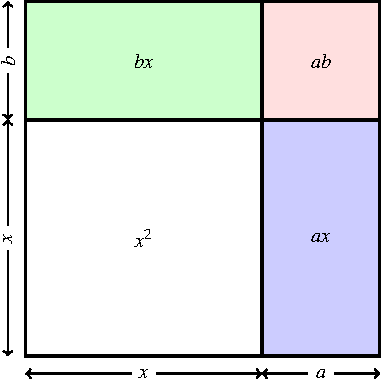
\includegraphics[scale=1.1]{image/08/quadratic-as-square.pdf}
\caption{%%
  The quadratic function $f(x) = (x + \alpha)(x + \beta)$ can be
  interpreted as a rectangle whose base and height have lengths
  $x + \alpha$ and $x + \beta$, respectively.
}
\label{fig:quadratic_as_rectangle}
\end{figure}

The obvious answer is that
\Expression{eqn:monic_quadratic_function_factored} gives you the
factored form of the quadratic function
%%
\begin{equation}
\label{eqn:monic_quadratic_function_roots}
f(x)
=
x^2 + (\alpha + \beta)x + \alpha\beta.
\end{equation}
%%
One factor is $x + \alpha$, the other factor is $x + \beta$, and
therefore the roots of $f(x)$ are $x = -\alpha$ and $x = -\beta$.  In
other words, when you have a quadratic function that can be written as
in \Expression{eqn:monic_quadratic_function}, you ask yourself: How do
I factorise the function so that I end up with something like
expressions~\eqref{eqn:monic_quadratic_function_factored}
or~\eqref{eqn:monic_quadratic_function_roots}?  If you compare
\Expressions{eqn:monic_quadratic_function}{eqn:monic_quadratic_function_factored},
you will notice that you have two equations:
%%
\begin{equation}
\label{eqn:monic_quadratic_function_factors_sum_product}
\alpha + \beta
=
b
%%
\qquad
\text{and}
\qquad
%%
\alpha\beta
=
c.
\end{equation}
%%
These equations tell you that you want two numbers $\alpha$ and
$\beta$ such that when they are added together you get $b$ and when
they are multiplied together you get $c$.  The problem now is to
determine the values of $\alpha$ and $\beta$.  The examples below will
help to clarify the theory.  The above discussion is summarised in the
next theorem.

\begin{theorem}
Consider the quadratic function
$f(x) = x^2 + (\alpha + \beta)x + \alpha\beta$, where $\alpha$ and
$\beta$ are any real numbers.  Then $f(x)$ can be written in factored
form as $f(x) = (x + \alpha) (x + \beta)$ and the roots of $f(x)$ are
$x = -\alpha$ and $x = -\beta$.
\end{theorem}

\begin{example}
\label{eg:factorise_monic_a1_b2_c6}
Consider the function $f(x) = x^2 + 5x + 6$.  Factorise $f(x)$ and
check your result.
\end{example}

\begin{solution}
The function $f(x)$ has the form similar to
\Expression{eqn:monic_quadratic_function} so you should consider the
equations
in~\eqref{eqn:monic_quadratic_function_factors_sum_product}.  That is,
you want two numbers $\alpha$ and $\beta$ whose sum is $5$ and whose
product is $6$.  You need to know the integer factors of $6$.  The
positive factors of $6$ are $1$, $2$, $3$, and $6$.  Among these
factors, choose two that sum to $5$ and have a product of $6$.  The
required factors are $2$ and $3$ because $2 + 3 = 5$ and
$2 \times 3 = 6$.  Therefore $f(x)$ can be written in factored form as
$f(x) = (x + 2) (x + 3)$.  You can check your result by using the
distributive laws to expand the multiplication.  Doing so produces
%%
\begin{align*}
(x + 2) (x + 3)
&=
x(x + 3) + 2(x + 3) \\[4pt]
&=
x^2 + 3x + 2x + 6 \\[4pt]
&=
x^2 + 5x + 6
\end{align*}
%%
which is the same as the definition of $f(x)$.
\end{solution}

\begin{exercise}
Factorise the function $f(x) = x^2 + 7x + 12$ and check your result.
\end{exercise}

\ifbool{showSolution}{
\begin{solution}
You want two numbers that sum to $7$ and have a product of $12$.  The
integer factors of $12$ are
\[
\sextuple{1}{2}{3}{4}{6}{12}
\]
among which $3$ and $4$ are the required integers.  Thus you have the
factored form $f(x) = (x + 3) (x + 4)$.  To check your result, use the
distributive laws to expand the multiplication:
%%
\begin{align*}
(x + 3) (x + 4)
&=
x(x + 4) + 3(x + 4) \\[4pt]
&=
x^2 + 4x + 3x + 12 \\[4pt]
&=
x^2 + 7x + 12.
\end{align*}
%%
The latter is the same as the definition of $f(x)$.
\end{solution}
}{}

\begin{example}
Consider the function $g(x) = 2x^2 + 16x + 30$.  Factorise the
function and check your result.
\end{example}

\begin{solution}
The function $g(x)$ looks like it is different from
\Expression{eqn:monic_quadratic_function}, but not really.  The trick
is to write $g(x)$ in such a way that allows you to use the technique
explained in \Example{eg:factorise_monic_a1_b2_c6}.  Note that each of
the three terms in $g(x)$ has a common factor, namely $2$.  Factoring
out the $2$ and $g(x)$ can be written as
\[
g(x)
=
2 (x^2 + 8x + 15).
\]
The function $h(x) = x^2 + 8x + 15$ has a form similar to
\Expression{eqn:monic_quadratic_function} so you can use the technique
in \Example{eg:factorise_monic_a1_b2_c6}.  You want two numbers that
add up to $8$ and have a product of $15$.  The positive integer
factors of $15$ are
\[
\quadruple{1}{3}{5}{15}
\]
among which $3$ and $5$ are the required integers.  Now write $h(x)$
in the factored form $h(x) = (x + 3) (x + 5)$ and therefore $g(x)$ can
be written in the factored form
\[
g(x)
=
2 (x + 3) (x + 5).
\]
To check your result, use the distributive laws to expand the
multiplication:
%%
\begin{align*}
2 (x + 3) (x + 5)
&=
2 \bigparen{x(x + 5) + 3(x + 5)} \\[4pt]
&=
2 \bigparen{x^2 + 5x + 3x + 15} \\[4pt]
&=
2 (x^2 + 8x + 15) \\[4pt]
&=
2x^2 + 16x + 30.
\end{align*}
%%
The latter expression is the same as how $g(x)$ was originally
defined.
\end{solution}

\begin{exercise}
Factorise the function $g(x) = 3x^2 + 15x + 18$ and check your
result.
\end{exercise}

\ifbool{showSolution}{
\begin{solution}
The trick is to write $g(x)$ in a form similar to
\Expression{eqn:monic_quadratic_function}.  Doing so would allow you
to use the technique explained in
\Example{eg:factorise_monic_a1_b2_c6}.  Each of the three terms in
$g(x)$ has $3$ as a common factor.  Hence $g(x)$ can be written as
\[
g(x)
=
3 (x^2 + 5x + 6).
\]
Since $h(x) = x^2 + 5x + 6$ is the same as the function in
\Example{eg:factorise_monic_a1_b2_c6}, then you have the factored form
$h(x) = (x + 2) (x + 3)$ and therefore $g(x)$ has the factored form
\[
g(x)
=
3 (x + 2) (x + 3).
\]
Use the distributive laws to expand the multiplication and you should
get the original expression for $g(x)$.
\end{solution}
}{}

\begin{example}
Factorise $f(x) = x^2 - 2x + 1$ and check your result.
\end{example}

\begin{solution}
You need to be careful about the negative sign.  The function $f(x)$
has a form similar to \Expression{eqn:monic_quadratic_function}.  You
require two numbers that sum to $-2$ and have a product of $1$.  Since
there is a negative sign, you must consider all integer factors of
$1$, both the positive and negative factors.  The positive factor of
$1$ is $1$ itself.  Now multiply each positive factor by $-1$ to get
the negative factors.  So multiplying $1$ by $-1$ results in $-1$.
Then the factors of $1$ are
\[
\pair{-1}{1}.
\]
The required integers are $-1$ and $-1$ again because you have the sum
\[
(-1) + (-1)
=
-2
\]
and the product $(-1) \times (-1) = 1$.  Now write $f(x)$ in the
factored form
\[
f(x)
=
(x - 1)^2.
\]
To check your result, use the distributive laws to expand the
multiplication:
%%
\begin{align*}
(x - 1)^2
&=
(x - 1) (x - 1) \\[4pt]
&=
x(x - 1) - 1(x - 1) \\[4pt]
&=
x^2 - x - x + 1 \\[4pt]
&=
x^2 - 2x + 1.
\end{align*}
%%
The latter expression is the same as the original definition of
$f(x)$.
\end{solution}

\begin{exercise}
Factorise $f(x) = -x^2 + 1$ and check your result.
\end{exercise}

\ifbool{showSolution}{
\begin{solution}
Note that the function $f(x)$ can be written as
\[
f(x)
=
-(x^2 - 1)
=
-(x^2 + 0 \cdot x - 1).
\]
Consider the function $g(x) = (x^2 + 0 \cdot x - 1)$.  You want two
numbers that sum to zero and have a product of $-1$.  The integer
factors of $-1$ are
\[
\pair{-1}{1}.
\]
Among these factors, $-1$ and $1$ are the required numbers because you
have the sum $-1 + 1 = 0$ and the product $(-1) \times 1 = -1$.  Now
write $g(x)$ in the factored form $g(x) = (x - 1) (x + 1)$ and
therefore $f(x)$ can be written in factored form as
\[
f(x)
=
-(x - 1) (x + 1).
\]
Use the distributive laws to expand the multiplication in the last
expression:
%%
\begin{align*}
-(x - 1)(x + 1)
&=
-\bigparen{x(x + 1) - 1(x + 1)} \\[4pt]
&=
-(x^2 + x - x - 1) \\[4pt]
&=
-(x^2 - 1) \\[4pt]
&=
-x^2 + 1.
\end{align*}
%%
The latter expression is the same as the original definition of
$f(x)$.
\end{solution}
}{}


%%%%%%%%%%%%%%%%%%%%%%%%%%%%%%%%%%%%%%%%%%%%%%%%%%%%%%%%%%%%%%%%%%%%%%%%%%%

\section{Completing the square}

\begin{figure}[!htbp]
\centering
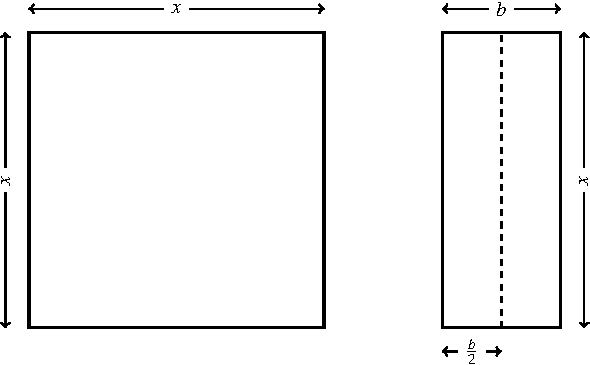
\includegraphics[scale=1.1]{image/10/complete-square-a1-c0.pdf}
\caption{%%
  The quadratic function $f(x) = x^2 + bx$ can be visualised as a
  square plus a rectangle.  The square has a side length of $x$, hence
  the area of the square is $x^2$.  The rectangle has a width of $b$
  and a height of $x$, so the rectangle has an area of $bx$.  Thus
  $f(x)$ can be interpreted as the area of a square plus the area of a
  rectangle.  The rectangle can be cut in half along the dashed line
  as shown.  Each half has a width of $b/2$ and a height of $x$.
}
\label{fig:special_complete_square_square_plus_rectangle}
\end{figure}

\begin{figure}[!htbp]
\centering
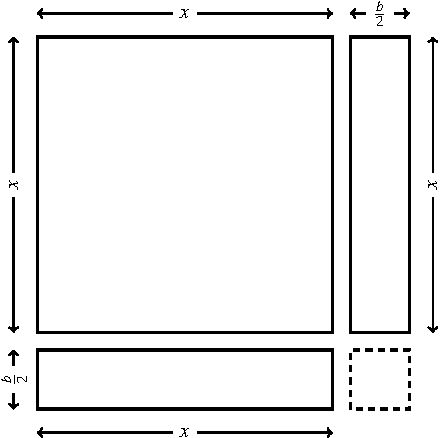
\includegraphics[scale=1.1]{image/10/complete-square-a1-c0_halfb.pdf}
\caption{%%
  The quadratic function $f(x) = x^2 + bx$ can be visualised as a
  square plus a rectangle.  The rectangle is cut in half.  One half is
  arranged to the right of the square.  The other half is arranged
  underneath the square.  Now you have a shape that is nearly like a
  square.  The small dashed square in the lower right is what is
  missing to make a complete square.
}
\label{fig:}
\end{figure}

\end{document}
